\documentclass[11pt,a4paper]{article}

\usepackage[margin=0.92in,top=1.02in,bottom=1.02in]{geometry}
\usepackage{amsmath,amssymb,mathtools}
\usepackage{booktabs,array}
\usepackage{graphicx}
\usepackage{xcolor}
\usepackage{xeCJK}
\xeCJKsetup{CJKspace=true}
\usepackage[most]{tcolorbox}
\usepackage{fancyhdr}
\usepackage{titlesec}
\usepackage{hyperref}

\setCJKmainfont[BoldFont={NanumMyeongjoExtraBold}]{Nanum Myeongjo}
\setCJKsansfont{Apple SD Gothic Neo}
\linespread{1.26}
\setlength{\parskip}{0.36em}
\setlength{\parindent}{0pt}
\renewcommand{\figurename}{\sffamily\bfseries 그림}
\renewcommand{\tablename}{\sffamily\bfseries 표}

\definecolor{navy}{HTML}{0F172A}
\definecolor{royal}{HTML}{1B5E7A}
\definecolor{teal}{HTML}{0D9488}
\definecolor{crimson}{HTML}{B23A2A}
\definecolor{amber}{HTML}{B45309}
\definecolor{softbg}{HTML}{F8FAFC}
\definecolor{softteal}{HTML}{F0FDFA}
\definecolor{softamber}{HTML}{FFFBEB}

\hypersetup{
  colorlinks=true,
  linkcolor=royal,
  urlcolor=royal,
  pdftitle={1943년 소련의 회전 팽이 방정식에서 발굴한 '파동 블랙홀'의 비밀}
}

\titleformat{\section}
  {\sffamily\Large\bfseries\color{navy}}
  {\textcolor{teal}{\thesection.}}{0.6em}{}
  [\vspace{2pt}\titlerule]

\titleformat{\subsection}
  {\sffamily\large\bfseries\color{royal}}
  {\thesubsection}{0.4em}{}

\pagestyle{fancy}
\fancyhf{}
\fancyhead[L]{\sffamily\footnotesize\color{gray} Project ReMath · 수학 고고학 특집 해설 (Study \#03)}
\fancyhead[R]{\sffamily\footnotesize\color{gray} 1943년 소련의 회전 팽이 방정식에서 발굴한 `파동 블랙홀'의 비밀}
\fancyfoot[C]{\sffamily\small\thepage}
\renewcommand{\headrulewidth}{0.4pt}

\newtcolorbox{wowbox}[1]{
  enhanced,
  colback=softteal,
  colframe=teal,
  boxrule=0.9pt,
  arc=3pt,
  left=10pt,right=10pt,top=7pt,bottom=7pt,
  fonttitle=\sffamily\bfseries,
  title={#1}
}

\newtcolorbox{storybox}[1]{
  enhanced,
  colback=softamber,
  colframe=amber,
  boxrule=0.9pt,
  arc=3pt,
  left=10pt,right=10pt,top=7pt,bottom=7pt,
  fonttitle=\sffamily\bfseries,
  title={#1}
}

\begin{document}

\begin{center}
  {\sffamily\footnotesize\bfseries\color{teal} MATHEMATICAL ARCHAEOLOGY · 수학 고고학 특집 리포트}\\[0.55em]
  {\sffamily\huge\bfseries\color{navy} 1943년 소련의 회전 팽이 방정식에서\\[0.18em] 발굴한 `파동 블랙홀'의 비밀}\\[0.5em]
  {\sffamily\large\color{darkgray} 종이 한 장 기울기의 대붕괴, 모래알 모서리 절단, 완벽 은폐 불가능 정리, 그리고 1000각형 대 1002각형의 역설}\\[0.9em]
  {\sffamily\small Project ReMath \quad|\quad 2026년 11월 24일}\\[0.25em]
  {\footnotesize\color{gray} 원전 아카이브: Sobolev (1954), Aleksandryan (1960), Zelenyak (1965), Fokin (2001--2002) (Math-Net.Ru)\\기계 검증: Lean~4.36.0 (공개 정리 125개·그중 주요 정리 40개, \texttt{sorry} 0개)}
\end{center}

\vspace{0.35em}

\begin{tcolorbox}[colback=softbg,colframe=navy,boxrule=0.7pt,arc=3pt,left=12pt,right=12pt,top=8pt,bottom=8pt]
\textbf{\sffamily 이 글에서 만날 4가지 수학적 반전 한눈에 보기}\\[0.25em]
1943년 소련의 액체 공동 회전 팽이 연구에서 출발한 \textbf{소볼레프 방정식}은 오늘날 \textbf{지구 액체 외핵·목성의 회전 유체}(관성파)와, 축을 맞바꾼 대응 구조로 \textbf{지구의 깊은 바다(성층 해양 내부파)} 속 파동을 기술한다. 보통의 빛이나 소리와 달리 이 파동은 벽의 기울기를 무시하고 \textbf{나침반처럼 고정된 각도로만 반사}되기 때문에, 물탱크의 모양을 조금만 건드려도 유입 영역 안의 파동 광선들을 1차원 닫힌 고리(\textbf{파동 블랙홀}, Wave Attractor)로 기하급수적으로 압축한다. 소련 알렉산드랸--젤레냐크--포킨 학파의 잊힌 원전을 발굴해 현대 동역학·기계증명(Lean~4)과 결합한 결과, 다음 네 가지 놀라운 정리가 드러났다:
\textbf{[반전 1]} 똑바른 정사각형 물탱크는 블랙홀 진동수 비율이 $0\%$이지만, \textbf{종이 한 장 두께($0.001^\circ$)}만 기울여도 그 비율이 순식간에 \textbf{$99.998\%$}로 폭등하며, $22.5^\circ$에서 마지막 정상파가 완전히 소멸한다 ·
\textbf{[반전 2]} 정사각형을 기울이지 않고 한쪽 모서리만 \textbf{모래알만큼} 깎아 넓이를 $0$으로 줄여 나가도, 블랙홀 진동수 비율의 극한 하한은 영구히 \textbf{$17.805\%$} 이상에 머문다(깎은 면적 $0.00019\%$에서 이미 $39{,}797$쌍, 총 $79{,}594$개 증명 구간이 $17.728\%$를 달성) ·
\textbf{[반전 3]} 4회 반사(주기~2) \textbf{끌림(어트랙터)} 고리와 정상파가 공존하려면 최소 \textbf{6각형} 물탱크가 필요하지만, 정상파는 \textbf{결코 블랙홀 고리의 눈을 피해 숨을 수 없다(고리 위 최대 진폭 최소 $50\%$ 강제 탐지)} ·
\textbf{[반전 4]} 원판과 눈으로 구별조차 안 되는 꼭짓점 정렬 \textbf{정1000각형}은 정중앙 진동수에서 무한히 많은 정상파를 지키지만, 변을 딱 두 개 더한 \textbf{정1002각형}은 그 즉시 \textbf{500개의 파동 블랙홀}로 산산조각 난다!
\end{tcolorbox}

\section{프롤로그: 1943년 소련의 회전 팽이와 지구 바다의 `나침반 파동'}

바이올린 현을 튕기거나 네모난 물그릇을 흔들면, 파동은 그릇 전체를 고르게 채우며 우아한 \textbf{정상파(standing wave)}를 만든다. 그릇을 살짝 기울이거나 모서리를 아주 조금 다듬더라도, 음높이가 미세하게 변할 뿐 정상파 자체는 멀쩡히 살아남는다는 것이 우리가 아는 상식이다.

그런데 물탱크가 회전하고 있거나(지구 액체 외핵, 목성의 대기), 아래쪽은 차갑고 무거운 바닷물·위쪽은 따뜻하고 가벼운 바닷물로 층이 나뉘어 있다면(\textbf{성층 해양의 내부파}) 이야기가 완전히 달라진다. 제2차 세계대전이 한창이던 1943년, 소련의 수학자 \textbf{세르게이 소볼레프(S.~L.~Sobolev)}는 액체가 담긴 회전 대칭 팽이의 동역학적 안정성을 분석하면서(내부 유체 방정식 자체는 1885년 푸앵카레가 이미 적었지만, 소볼레프가 비코발렙스키형 초기-경계값 문제와 힐베르트 공간 이론을 체계화했다) 다음 편미분방정식을 정립했다:
\begin{equation}\label{eq:kr-sobolev}
  \partial_t^2 \Delta u + \partial_z^2 u = 0 \qquad (\text{진동수 } \lambda\text{에서}\;\; (1-\lambda^2)u_{zz} - \lambda^2 u_{xx} = 0).
\end{equation}

\begin{storybox}{수학 고고학 노트: 알렉산드랸(1960)에서 마스--람(1995)까지, 35년을 앞선 소련 학파}
소볼레프가 1943년에 완성한 액체 공동 회전 팽이 논문은 1960년에 출판되었고, 편미분방정식 본편은 1951년 10월 2일 모스크바 수학회 강연(1952년 게재)을 거쳐 1954년 기념비적 논문으로 세상에 나왔다. 그의 제자 \textbf{라파엘 알렉산드랸(R.~A.~Aleksandryan, 아르메니아 예레반)}은 프리츠 존(F.~John, 1941) 등의 선구적 연구를 발전시켜 1949년 박사논문과 1960년 《모스크바 수학회보》 대논문에서 이 스펙트럼 문제를 \textbf{`경계면 위 반사 사상(원 위상동형사상)'}으로 환원하는 체계를 정립했고, 원판에서는 다항식 정상파가 완전 기저를 이루지만 원판에 임의로 가까운 매끄러운 영역 중에도 준주기성이 깨지는 해가 존재함을 최초로 구성해 보였다. 뒤이어 시베리아 노보시비르스크의 \textbf{타데이 젤레냐크(T.~I.~Zelenyak, 1965--1970)}와 \textbf{미하일 포킨(M.~V.~Fokin, 1981--2002)}이 이 계보를 이어갔지만, 핵심 단행본과 논문 상당수가 영어로 번역되지 못한 채 철의 장막 뒤에 머물렀다. 알렉산드랸의 1960년 논문으로부터 35년 뒤(중간에 스튜어트슨(K.~Stewartson, 1972)이 반사 광선의 극한 고리 수렴을 기술한 바 있다)인 1995년, 네덜란드 해양학자 마스(L.~Maas)와 람(F.~Lam)이 파동 어트랙터의 기하학을 본격 재발견했고, 1997년 \textbf{마스·베니엘리·소메리아·람}이 성층 수조 실험으로 이를 직접 관측해 《네이처》에 발표하면서 현대 수학·해양물리학의 뜨거운 주제로 되살아났다.
\end{storybox}

소볼레프 방정식이 보통의 소리·빛과 결정적으로 다른 이유는 딱 하나다. 거울에 비친 빛은 벽의 수직선 기준으로 `입사각 $=$ 반사각'을 따르지만, 연직축 회전 유체의 관성파는 \textbf{벽이 몇 도로 기울어져 있든 상관없이 오직 진동수 $\lambda = \omega/f = \cos\theta$가 정한 고정된 나침반 각도 $\pm\theta$로만 튕겨 나간다}(성층 해양의 내부 중력파는 수평·수직 축을 맞바꾼 대응 관계 $\omega/N = \sin\theta$, 즉 스펙트럼 매개변수 $1 - E$에 해당한다; 그림~\ref{fig:kr1}A).

그 결과 비임계 경사벽에 파동 다발이 압축 방향(focusing direction)으로 부딪히면 반사된 다발의 폭이 확 줄어들며 에너지가 좁은 띠로 몰린다(반대 시간 방향의 광선은 같은 벽에서 팽창한다). 이러한 압축이 순환을 따라 누적되면, 특정 \textbf{파동 블랙홀}의 유입 영역(basin) 안에서 출발한 기하 광선들은 결국 그 1차원 닫힌 고리 위로 지수함수적으로 빨려 들어가 집중된다.

\begin{figure}[ht]
\centering
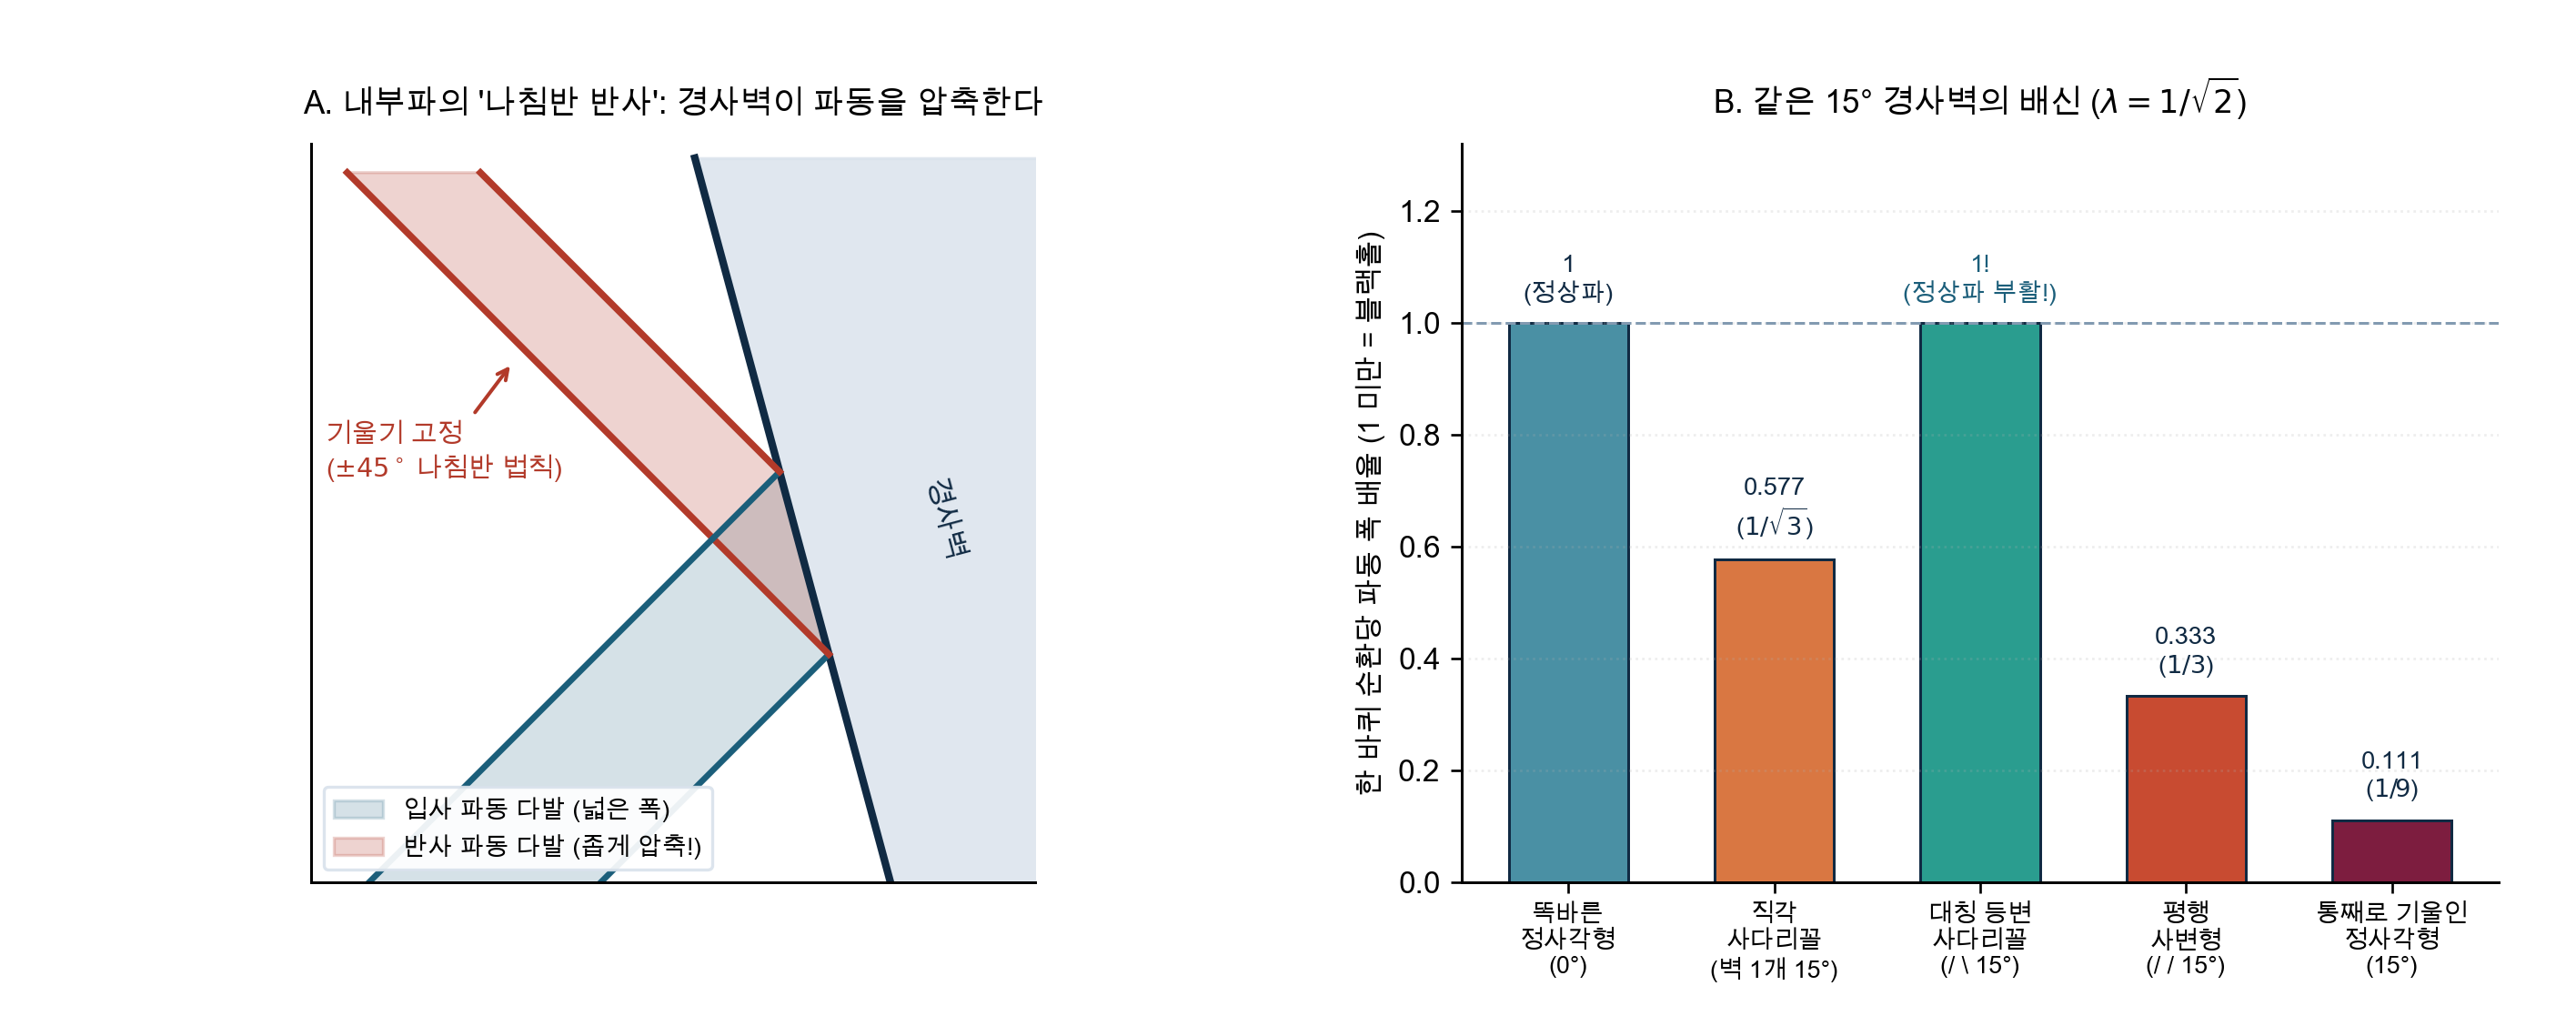
\includegraphics[width=\textwidth]{figs/kr_fig1_compass_and_two_walls.png}
\caption{\textbf{A.} 내부파의 `나침반 반사': 비임계 경사벽에 압축 방향으로 부딪혀도 파동의 기울기가 $\pm 45^\circ$로 고정되므로, 넓은 입사 다발이 반사 후 좁게 압축된다. \textbf{B.} 밑변이 수평인 네 사각형(실험실 높이 $H =$ 중앙 폭 $W$)과 몸체 좌표 정사각형을 통째로 $15^\circ$ 기울인 다섯 번째 물탱크의 극적 반전($\lambda = 1/\sqrt{2}$): 벽 하나만 기울이면 $1/\sqrt{3}$로 압축되지만, 반대편 벽을 대칭으로 기울인 등변 사다리꼴은 압축이 완벽히 상쇄되어 정상파($1$)가 부활한다! 반면 나란히 기울인 평행사변형은 $1/3$, 통째로 기울인 정사각형은 $1/9$로 압축력이 제곱된다.}
\label{fig:kr1}
\end{figure}

그렇다면 경사벽이 많을수록 무조건 더 강한 블랙홀이 생길까? 아니다! 그림~\ref{fig:kr1}B의 \textbf{`다섯 물탱크의 배신'}을 보라. 밑변이 수평이고 높이와 중앙 폭이 같은($H = W$) 똑바로 선 정사각형 물탱크($0^\circ$)의 한쪽 벽을 $15^\circ$ 기울여 직각 사다리꼴을 만들면, 정중앙 진동수($\lambda = 1/\sqrt{2}$, $\pm 45^\circ$ 파동)에서 파동 폭이 한 바퀴 돌 때마다 $1/\sqrt{3} \approx 0.577$배로 압축된다. 그런데 반대쪽 벽마저 마주 보게 $15^\circ$ 기울여 \textbf{대칭 등변 사다리꼴}을 만들면? 놀랍게도 두 경사벽의 압축과 팽창이 정확히 맞물려 상쇄되면서 \textbf{배율이 다시 $1$로 돌아와 정상파가 완벽히 부활한다!} 반대로 두 벽을 같은 방향으로 나란히 기울여 \textbf{평행사변형}을 만들면 압축력이 제곱되어 $1/3$배, 정사각형 자체(몸체 좌표 $H_{\mathrm{body}} = W_{\mathrm{body}}$)를 아예 \textbf{통째로 $15^\circ$ 기울이면} 네 벽 모두가 합세해 한 바퀴마다 무려 \textbf{$1/9$배(9배 압축!)}로 파동을 으깨 버린다. 우리는 다섯 사각형 가족 전체의 정상파·블랙홀 판별법을 단 하나의 홀짝 법칙으로 통합 증명하고 핵심 대수 구조를 Lean~4로 기계 검증했다.

\section{반전 1 \& 2: 종이 한 장 기울기의 대붕괴와 모래알 모서리 절단}

똑바로 세운 정사각형 물탱크에서는 네 벽이 모두 수평·수직이라 나침반 반사가 보통 당구 반사와 똑같아진다. 그래서 파동 블랙홀이 생기는 진동수 비율은 \textbf{정확히 $0\%$}이며, 고전적인 사인($\sin$) 정상파들이 완전 기저를 이루며 탱크 전체를 평화롭게 지배한다.

이제 이 정사각형 물탱크 한쪽 밑에 \textbf{종이 한 장을 끼워 단 $0.001^\circ$만 기울여 보자.} 상식대로라면 블랙홀 진동수도 $0.001\%$쯤 아주 살짝 생길 것 같다. 하지만 우리가 증명한 정리는 정반대의 참사를 보여준다.

\begin{wowbox}{정리 (단일 기울어진 직사각형의 전측도 대붕괴와 $22.5^\circ$ 소멸 절벽)}
가로세로 비가 $R$인 어떤 직사각형 물탱크든, 각도 $\phi \in (0^\circ, 45^\circ)$로 \textbf{고정해 기울이는 순간} 전체 진동수 구간 $(0,1)$에서:
\begin{itemize}
  \item 똑바른 상태($0^\circ$)에서 $0\%$였던 블랙홀 진동수 비율이, 주기 파동 블랙홀 $\cos\phi - \sin\phi$와 꼭짓점 포획 $1 - \cos\phi + \sin\phi$로 나뉘어 합이 \textbf{정확히 $100\%$(르베그 측도 $1$)}로 불연속 도약한다! (단 $0.001^\circ$만 기울여도 주기 블랙홀이 즉시 \textbf{$99.998\%$}, 꼭짓점 포획이 나머지 $0.002\%$를 차지한다.)
  \item 블랙홀을 피해 살아남는 예외 진동수 집합(정상파 진동수 포함)은 소멸 절벽 바깥에서 비어 있지 않은 르베그 측도 $0$의 프랙털 칸토어 집합을 이루며, 그 하우스도르프 차원은 모든 $R > 0$에 대해 균일하게 $1$보다 작다(기울기 $15^\circ$ 이상에서는 엄밀한 정수 10제곱 계산으로 \textbf{차원 $\le 9/10$}을 증명!).
  \item 게다가 가로세로 비 $R$과 기울기 $\phi$가 $\cot(2\phi) \le R \le \tan(2\phi)$ 안에 들어가면 물탱크의 \textbf{모든 정상파가 단 하나도 남김없이 영구 소멸}한다($\sigma_p(T) = \varnothing$). 정사각형($R=1$)의 경우, 정확히 \textbf{$\phi = 22.5^\circ$}가 마지막 정상파가 숨을 거두는 절벽이다!
\end{itemize}
\end{wowbox}

이 결과는 최근 출판된 학술 논문(Y.~Zhang--A.~N.~Temnov, 2026)의 직사각형 공명 판별법이 양방향 모두 틀렸음도 정확히 반증한다. 예컨대 정사각형을 $\tan\phi = 1/3$($\approx 18.43^\circ$)만큼 기울이면 \textbf{정중앙 진동수($\lambda^2 = 1/2$)}에서 탱크 내부 좌표의 파동 기울기가 완벽한 유리수 $1/2$과 $-2$가 되지만, 실제로는 그 진동수에 정상파가 단 하나도 없고 같은 네 변을 반대 방향으로 도는 두 유향 고리(수축 배율 $1/16$의 블랙홀과 팽창 배율 $16$의 반발 고리)만 존재한다(Lean~4로 12개 경계 구간 전수 검증 완료).

\begin{figure}[ht]
\centering
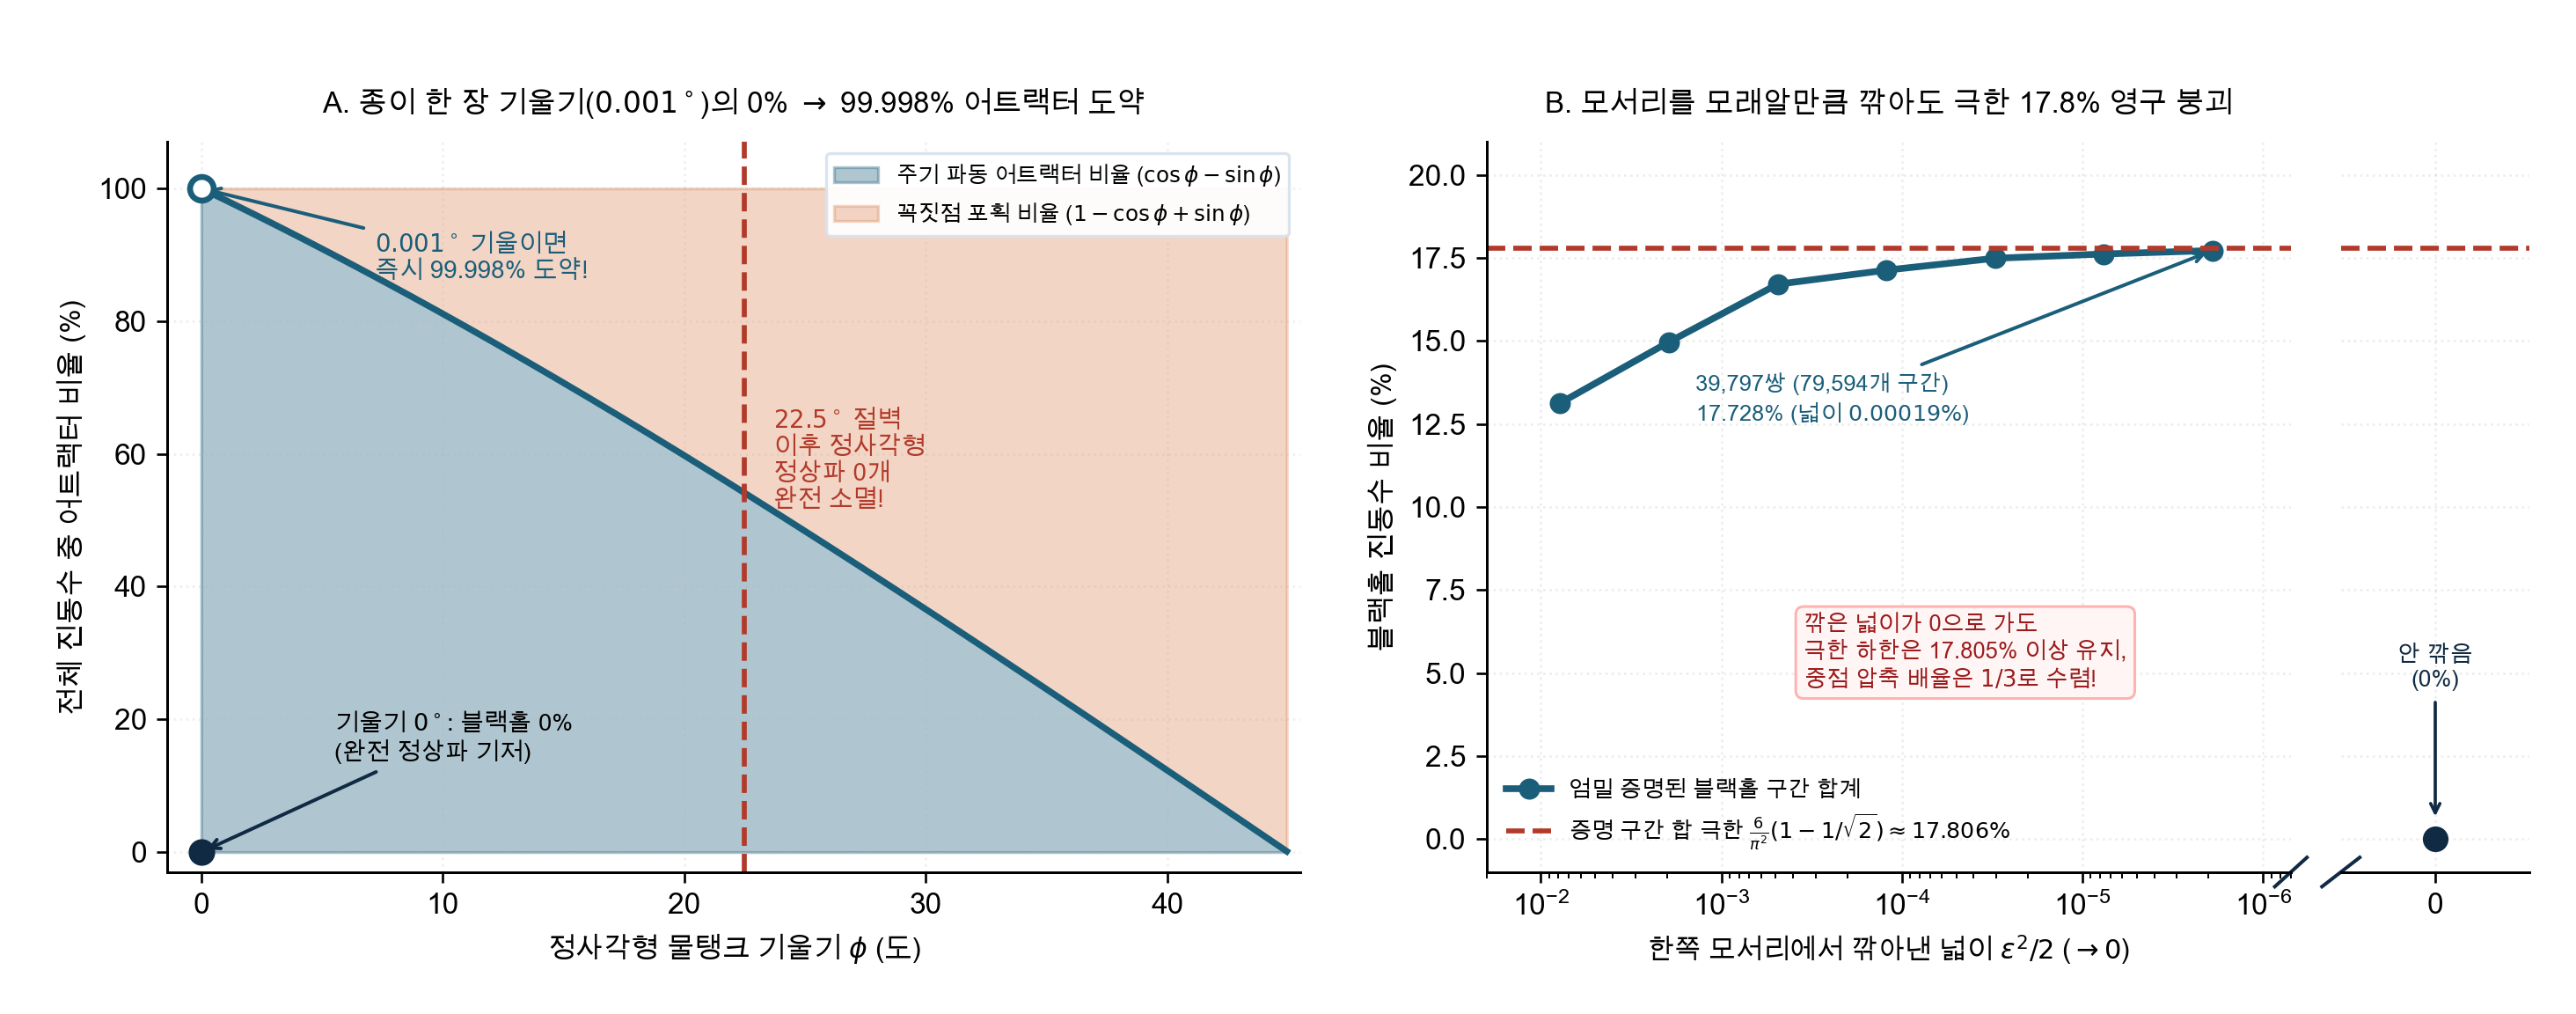
\includegraphics[width=\textwidth]{figs/kr_fig2_tilt_and_sand_chip.png}
\caption{\textbf{A.} 똑바른 정사각형($0^\circ$)은 완전한 정상파 기저를 갖고 블랙홀 비율이 $0\%$이지만, 단 $0.001^\circ$만 기울여도 주기 블랙홀($\cos\phi-\sin\phi$, 청색)이 즉시 $99.998\%$로 폭등한다. $22.5^\circ$ 절벽을 넘으면 정사각형의 정상파는 완전히 $0$개가 된다. \textbf{B.} 탱크를 기울이지 않고 한쪽 모서리만 면적 $\varepsilon^2/2$만큼 비스듬히 깎아 넓이를 $0$으로 줄여 나가면, 증명된 서로소 고원 합은 $C = \frac{6}{\pi^2}(1 - 1/\sqrt{2}) = 17.80577\ldots\%$로 수렴한다($\varepsilon = 1/512$, 깎은 면적 $0.00019\%$에서 $39{,}797$쌍, 총 $79{,}594$개 구간 합 $17.728\%$). 이는 전체 블랙홀 진동수 비율의 극한 하한이 적어도 $C$ 이상($\liminf_{\varepsilon\downarrow 0}|\mathcal{A}_\varepsilon|_\lambda \ge C > 17.805\%$)임을 증명하며, 안 깎은 정사각형($0\%$)과의 영구적 단절을 보장한다.}
\label{fig:kr2}
\end{figure}

더 기막힌 질문이 뒤따른다. ``그렇다면 물탱크를 기울이지 않고 똑바로 세워 둔 채, 한쪽 모서리만 아주 살짝---마치 모래알 하나 크기만큼만---비스듬히 깎아내면 어떨까?''

수평·수직 벽이 네 개 다 멀쩡히 남아 있으니, 깎아낸 삼각형 넓이 $\varepsilon^2/2$가 $0$에 가까워지면 블랙홀 비율도 $0\%$로 돌아갈 것 같다. 그러나 우리가 증명한 \textbf{미세 모서리 절단 정리}는 그 직관을 산산이 부순다(그림~\ref{fig:kr2}B).
\begin{itemize}
  \item 아무리 모서리를 작게 깎아도($u \le v$, $\tau = v/u$), $1 \le m < n$, $s_* = m/(n-u) < \tau$, $v + s_* u < 1/n$을 만족하는 서로소 정수 쌍 $(m,n)$마다 정확한 고원 $[m/n,\, s_*]$이 생긴다. 왼쪽 끝점 $s = m/n$에는 무한히 많은 정상파가 남아 있지만, 열린 내부 구간 $(m/n,\, s_*)$은 정규 파동 블랙홀(압축 배율 $(\tau-s)/(\tau+s)$), 오른쪽 끝점 $s_*$는 꼭짓점 순환 궤도로서 $(m/n,\, s_*]$ 전체에서 정상파가 완전히 사라진다.
  \item 심지어 모래알 크기가 줄어들수록 개별 고원은 좁아지지만 \textbf{고원의 개수 자체가 폭발적으로 늘어나고}($\varepsilon = 1/512$, 깎은 면적 $0.00019\%$일 때 이미 $s < 1$에 $39{,}797$개, 대칭 역수 쌍을 합쳐 총 \textbf{$79{,}594$개}의 서로소 증명 구간!), 각 블랙홀이 깎인 면을 딱 한 번 스칠 때의 압축 배율 $(1-s)/(1+s)$은 $\varepsilon$이 아무리 작아져도 줄어들지 않는다(대표 주기-3 고리의 깎인 면 중점 압축 배율 $(2-\varepsilon)/(6-\varepsilon)$은 $\varepsilon \downarrow 0$일 때 \textbf{정확히 $1/3$, 즉 3배 압축}으로 수렴!).
  \item 이 서로소 증명 구간들의 길이를 수론의 뫼비우스 반전 공식($6/\pi^2 = 1/\zeta(2)$)으로 합산하면, 모서리 절단 넓이가 $0$으로 향할 때 그 합은
  \[
    C = \frac{6}{\pi^2}\left(1 - \frac{1}{\sqrt{2}}\right) = 17.80577\ldots \%
  \]
  로 수렴한다($\varepsilon = 1/512$에서 이미 $17.728\%$ 달성). 따라서 전체 블랙홀 진동수 비율의 극한 하한은 적어도 $C$ 이상($\liminf_{\varepsilon \downarrow 0}|\mathcal{A}_\varepsilon|_\lambda \ge C > 17.805\%$)이다! 더 나아가 우리는 \textbf{전체 볼록 다각형 강성 정리}를 통해, 지구상의 모든 볼록 다각형 가운데 모든 진동수에서 파동 블랙홀과 꼭짓점 포획을 완전히 피하는 도형은 \textbf{오직 똑바로 선 직사각형 단 하나뿐}임을 최종 증명했다.
\end{itemize}

\section{반전 3: 정상파와 블랙홀의 공존, 그리고 `완벽 은폐 불가능 정리'}

그렇다면 하나의 물탱크 안에서 \textbf{같은 진동수}에 평화로운 정상파와 에너지 포식자 블랙홀이 \textbf{동시에 공존}할 수는 없을까?

우리가 증명한 기하학적 한계선은 놀랍도록 단호하다. \textbf{어떤 볼록 사각형에서도(직사각형·사다리꼴·마름모·임의의 볼록 사각형 모두) 정상파와 블랙홀은 결코 같은 진동수에 공존할 수 없다!} 4번 반사해 제자리로 돌아오는 \textbf{끌림(어트랙터) 닫힌 고리(주기~2)}와 정상파가 함께 살려면 \textbf{최소 6각형}이 필요하고, 점대칭 도형에서는 \textbf{최소 8각형}이 필요하다. 더 놀라운 점은, 변을 하나씩 추가할 때마다($k = m + 5$각형) 우리가 원하는 순서의 특성 반높이 $0 < r_1 < \dots < r_m < a$와 원하는 압축률 $\kappa_1, \dots, \kappa_m \in (0,1)$을 가진 \textbf{$m$개의 맞춤형 파동 블랙홀}을 자유자재로 심으면서도, 원래 있던 무한차원 정상파 공간과 그 파동 에너지를 단 $1\%$도 건드리지 않고 그대로 보존할 수 있다는 사실이다!

\begin{figure}[ht]
\centering
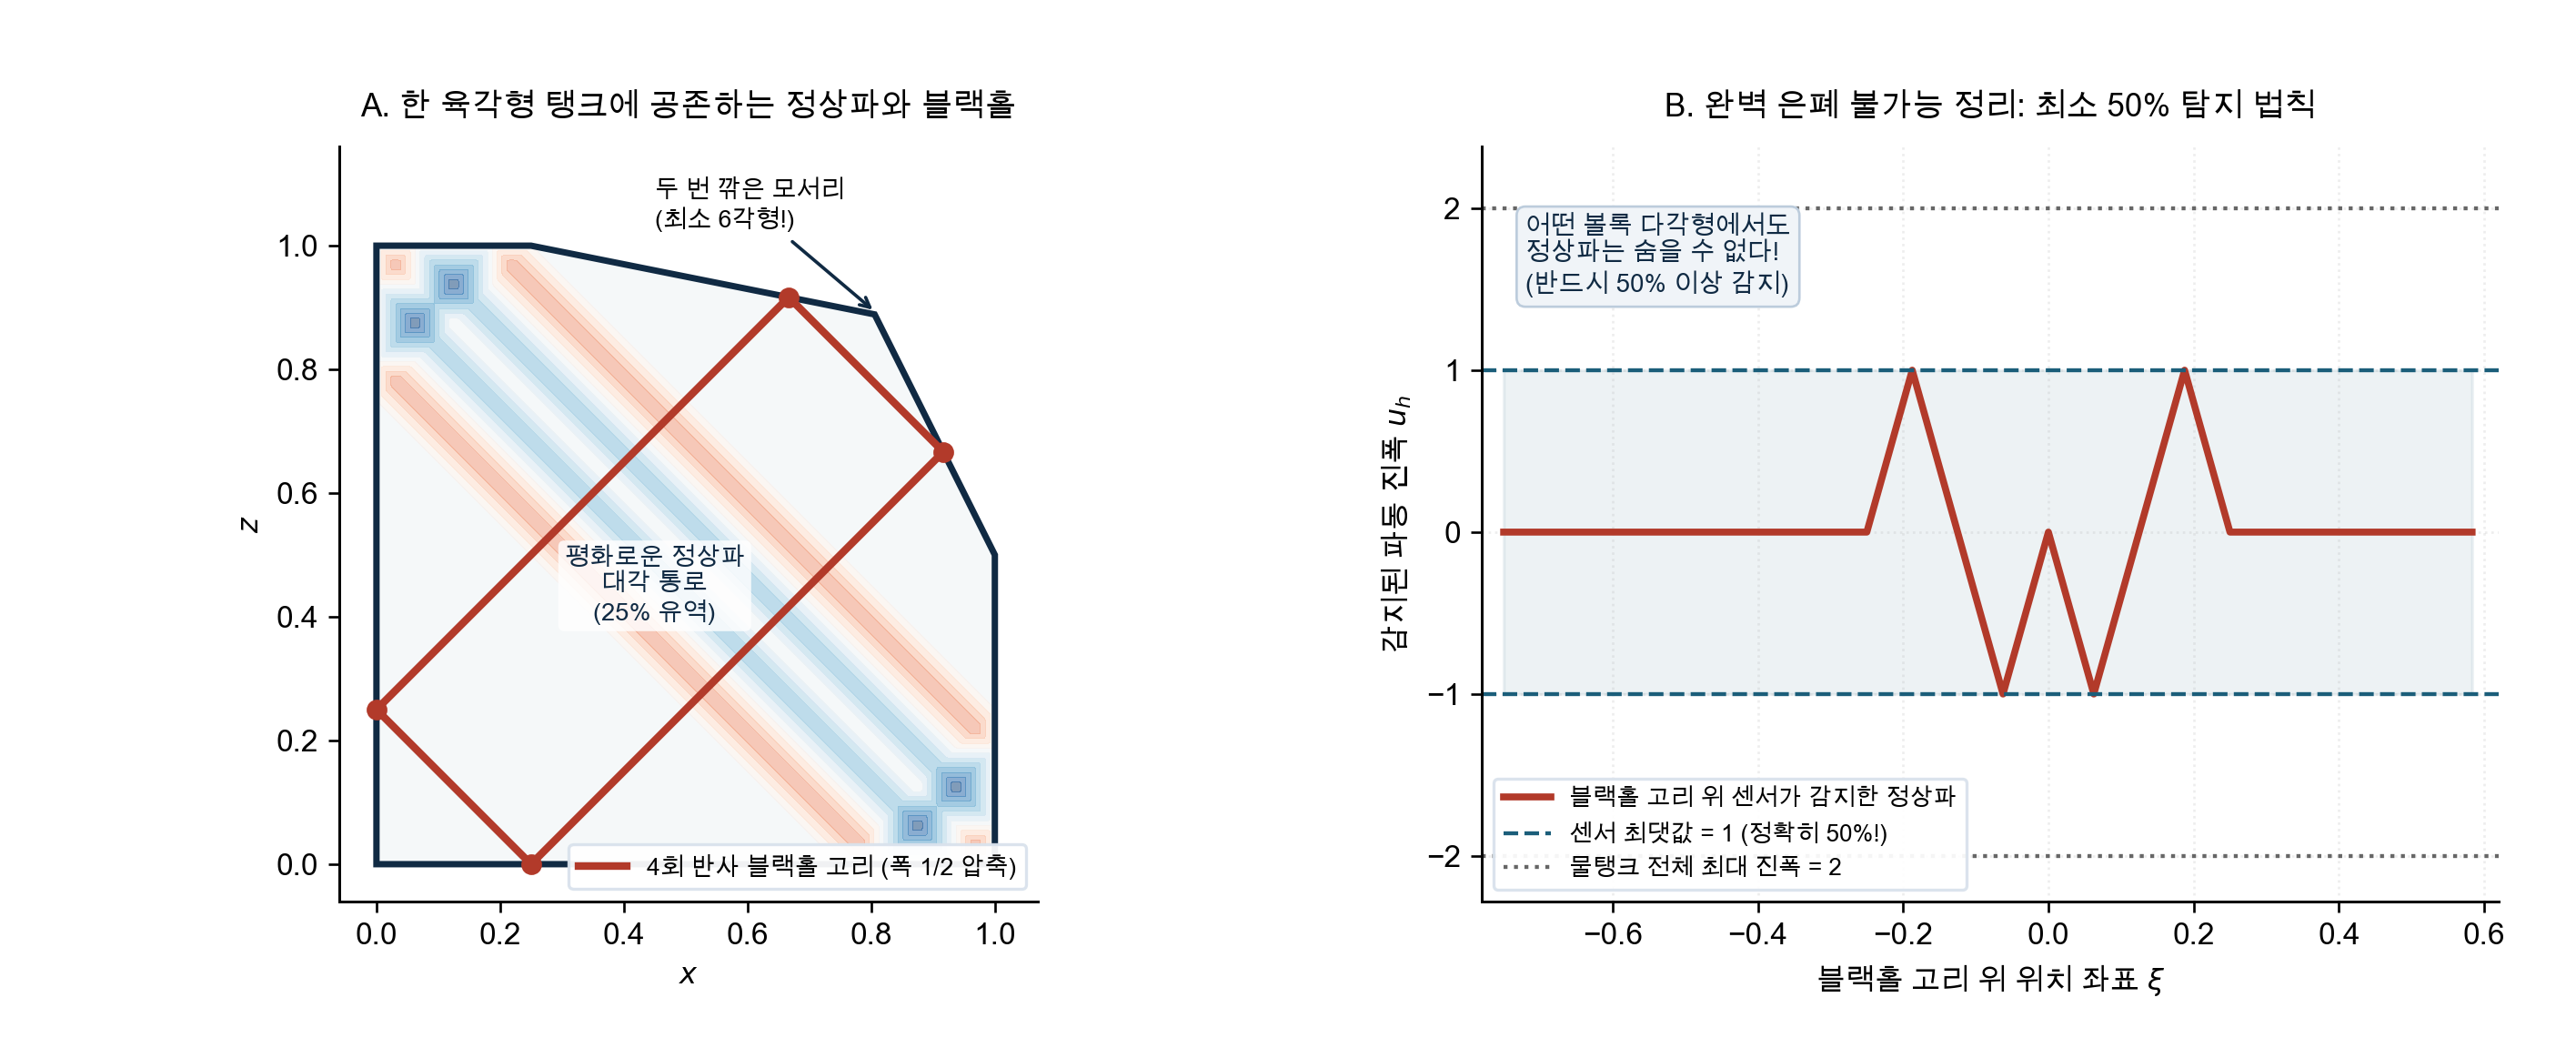
\includegraphics[width=\textwidth]{figs/kr_fig3_impossible_cloak_hexagon.png}
\caption{\textbf{A.} 정사각형의 오른쪽 위 모서리를 두 번 꺾어 깎아 만든 최소 주기-2 공존 6각형($\lambda = 1/\sqrt{2}$). 대각선 통로에는 무한히 많은 매끄러운 정상파가 살아 숨 쉬며, 파랑·주황 등고선은 같은 고유공간에 속하면서 하한 $50\%$를 정확히 달성하는 대표 유한에너지($H_0^1$) 조각별 선형 고유모드 $u_h$를 보여준다. 그 한가운데를 4회 반사 파동 블랙홀(붉은 고리, 한 바퀴마다 폭 $1/2$ 압축)이 관통한다. \textbf{B.} \textbf{완벽 은폐 불가능 정리}: 어떤 볼록 다각형에서도 정상파는 정규 주기 블랙홀 고리 전체에서 숨을 수 없다! 탱크 전체 최대 진폭이 $2$일 때, 블랙홀 고리 위에는 반드시 진폭이 $1$(정확히 $50\%$) 이상인 지점이 존재한다.}
\label{fig:kr3}
\end{figure}

여기서 물리학자라면 누구나 떠올릴 매력적인 상상이 있다. ``정상파가 블랙홀 고리를 피해 탱크 한쪽의 평화로운 구석 방에만 조용히 숨어 있으면 어떨까? 그러면 블랙홀 고리 전체를 따라 센서를 설치해도 정상파의 흔적이 어디에서도 보이지 않거나(항상 $0$), 아주 미미하게만 잡히지 않을까?''

이 상상은 수학적으로 \textbf{100\% 불가능하다!}(물론 고리 위 특정 한 점에서는 우연히 $0$이 읽힐 수 있지만, 고리 전체를 따라 숨는 일은 원천 봉쇄된다.) 우리가 증명한 \textbf{완벽 은폐 불가능 정리(Universal Half-Amplitude Uncloakability Theorem)}는 다음과 같은 단단한 법칙을 못 박는다.

\begin{wowbox}{정리 (완벽 은폐 불가능 정리: 최소 $50\%$ 강제 탐지 법칙)}
어떤 볼록 다각형 물탱크에서든(변이 6개든 100만 개든), 비특성 진동수에서 정상파 $u$와 정규 닫힌 주기 파동 블랙홀 고리 $\Gamma$가 공존한다면, 블랙홀 고리 위에서 관측되는 정상파의 \textbf{최대 진폭}은 \textbf{항상 물탱크 전체 최대 진폭의 절반($50\%$) 이상}이다(고리의 특정 한 점에서는 $0$이 될 수 있어도, 고리 전체를 따라 숨는 일은 불가능하다):
\[
  \|u\|_{L^\infty(\Gamma)} \;\ge\; \frac{1}{2}\,\|u\|_{L^\infty(\Omega)}.
\]
이 $50\%$ 하한은 더 이상 높일 수 없는 날카로운 상수이며, 그림~\ref{fig:kr3}의 최소 주기-2 공존 6각형에서 정확히 $50\%$(전체 최댓값 $2$, 블랙홀 위 관측 최댓값 $1$)로 달성된다!
\end{wowbox}

이유는 경이로운 위상 기하학 한 줄로 설명된다. 볼록 다각형 경계 위에서 서로 다른 닫힌 주기 궤도들은 반드시 \textbf{서로 엇갈리며 교차(interlacing)}할 수밖에 없다. 따라서 조르당 곡선 정리에 의해 정상파의 최대 진폭을 만드는 내부 궤도들과 블랙홀 고리 $\Gamma$는 탱크 내부에서 \textbf{반드시 정면으로 교차}해야 하며, 그 교차점에서 블랙홀 고리는 정상파가 가진 경계 진동폭의 최소 절반을 온몸으로 맞닥뜨리게 된다! 게다가 최소 6각형 공존 탱크에서 수평 특성 좌표($\eta \in [-1,1]$)를 균등하게, 좌우 출발 벽을 같은 확률로 골라 파동을 쏘아 보냈을 때, $25\%$는 정상파 통로에 남고, $50\%$는 중앙 블랙홀로 빨려 들며, 나머지 $25\%$는 두 번씩 건너뛴 반복($b^{2n}x$)이 정상파 통로의 경계 끝점으로, 즉 전체 궤도가 그 끝점의 주기-2 순환 고리로 수렴한다(시간 반전 대칭성이 양의 측도를 가진 끝점 수렴 구간의 존재를 강제하며, 반환 사상 계산이 그 정확한 비율 $25\%$를 결정한다).

\section{반전 4: 정1000각형 대 정1002각형의 역설과 팔각형 \texorpdfstring{$0.00001^\circ$}{0.00001도} 절벽}

이제 마지막 반전으로 넘어가자. 완벽한 원판 물탱크에서는 모든 파동이 평화로운 정상파로 분해된다(알렉산드랸, 1960). 그렇다면 변이 1000개나 되는 정다각형---눈으로 보면 원과 머리카락 굵기만큼도 구별할 수 없는 \textbf{정1000각형}과 \textbf{정1002각형}---은 둘 다 원판과 똑같이 평화로울까?

꼭짓점을 위쪽으로 똑바로 세운 두 정다각형(Paper~2의 $x$-축 기준 위상 규약으로는 $N=1000$이 $\phi = 0$, $N=1002$는 $\phi = h \bmod 2h$이며, $90^\circ$ 회전 대칭 덕분에 $E = 1/2$에서의 개수와 배율 집합은 $\phi = 0$ 기준과 완전히 동일하다)을 정중앙 진동수($\lambda = 1/\sqrt{2}$, $\pm 45^\circ$ 파동)에 나란히 올려놓으면 충격적인 분열이 벌어진다(그림~\ref{fig:kr4}A):
\begin{itemize}
  \item \textbf{정1000각형 ($N$이 8의 배수)}: $45^\circ$와 $135^\circ$ 반사선의 거울 대칭축이 다각형의 마주 보는 꼭짓점·변과 정확히 맞물리기 때문에, 모든 파동이 두 번 반사하면 정반대편 대칭점($b(p) = -p$)으로, 네 번 반사하면 제자리($b^2(p) = p$)로 돌아온다. 원판의 정중앙 \textbf{진동수}($E = 1/2$)가 단 한 치의 오차도 없이 살아남아 \textbf{무한히 많은 정확한 정상파}를 유지한다(단, 원판 다항식 $1-r^2$ 자체는 변 중점에서 $\sin^2(\pi/N)$만큼 어긋나므로 살아남는 것은 다각형 고유의 주기-2 정상파들이다).
  \item \textbf{정1002각형 ($N = 4m+2$)}: 변을 딱 두 개만 더했는데, 그 즉시 모든 벽이 $45^\circ$ 거울 대칭 격자에서 미세하게 어긋난다! 그 순간 정확한 정상파는 \textbf{단 하나도 남지 않고 $0$개로 전멸}하며, 탱크 내부는 무려 \textbf{500개의 파동 블랙홀}로 쪼개진다!
\end{itemize}

\begin{figure}[ht]
\centering
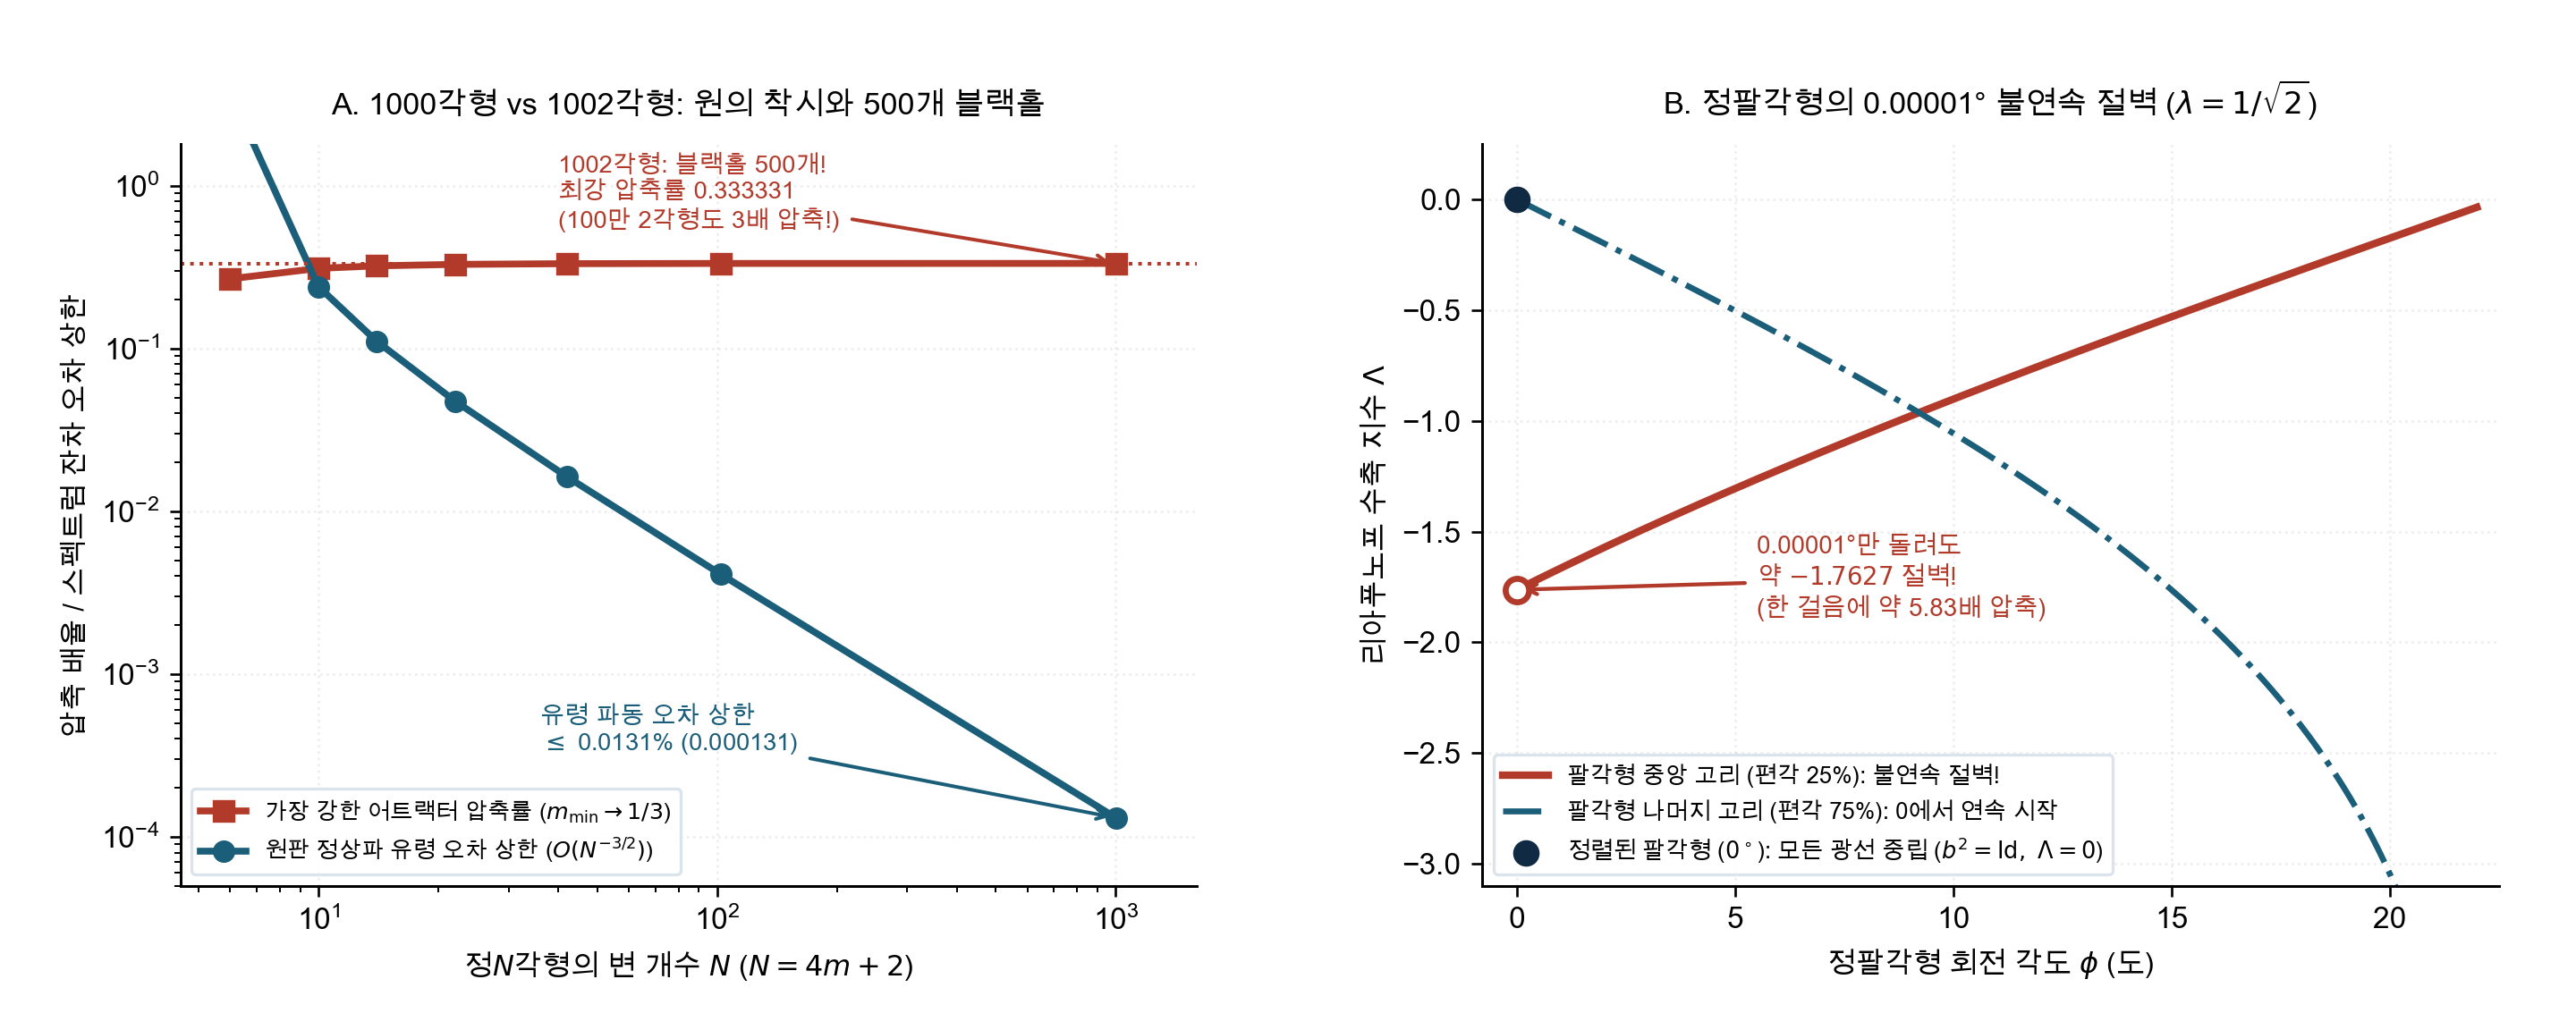
\includegraphics[width=\textwidth]{figs/kr_fig4_1000_vs_1002_and_octagon.png}
\caption{\textbf{A.} 정1002각형($N=4m+2$)의 이중 얼굴: 변의 개수 $N$이 $1{,}000{,}002$로 커져도 가장 강력한 블랙홀의 한 걸음 압축 배율 $m_{\min} = (2\cos(\pi/N)-1)/(2\cos(\pi/N)+1)$은 항상 $1/3$ 미만으로 눌린 채 \textbf{$1/3$(3배 압축)}로 수렴한다($N=1002$에서 $0.333331$, 붉은 선). 그런데도 원판 정상파 $1-r^2$를 보정한 `유령 파동'의 상대 오차 \textbf{상한}은 $N^{-3/2}$로 추락해 정1002각형에서 \textbf{$0.0131\%$ 이하}($\le 0.000131$)에 불과하다(파란 선)! \textbf{B.} 정팔각형의 불연속 절벽: 정렬된 $0^\circ$에서는 모든 기하 광선이 중립 주기-2 궤도($b^2 = \mathrm{Id}$, $\Lambda = 0$)를 이루며 무한차원 정상파 공간이 존재하지만, 단 $0.00001^\circ$만 돌려도 편각 기준 $25\%$ 영역이 즉시 한 걸음당 약 $5.83$배 압축($\Lambda \approx -1.7627$, 극한값 $-2\log(1+\sqrt{2})$)이라는 깊은 절벽으로 추락한다.}
\label{fig:kr4}
\end{figure}

더 어지러운 역설은 정1002각형의 변을 $100{,}002$개, $1{,}000{,}002$개($N = 4m+2 \to \infty$)로 계속 늘릴 때 벌어진다.
\begin{enumerate}
  \item 경계 호의 길이를 따라 균등하게 파동을 쏘았을 때 대다수 파동이 겪는 압축 지수 $\ell_N$은 $1/N$ 크기로 서서히 약해지며, 재조정량 $-N\ell_N$이 $2\pi/\sin(\pi U)$ 보편 분포($U \sim \mathrm{Unif}(0,1)$는 $(0,1)$ 균등 확률변수)로 \textbf{분포 수렴}한다(유한한 $N$에서는 이산 분포).
  \item 그러나 탱크 안에서 \textbf{가장 강력한 블랙홀}의 한 걸음 압축 배율은 $N=1002$에서 $0.333331$, $N=1{,}000{,}002$가 되어도 영원히 \textbf{$1/3$(한 걸음에 3배 압축!)} 아래에 못 박혀 사라지지 않는다!
  \item 그런데 놀랍게도, 정확한 정상파가 $0$개인 그 정1002각형 위에서 원판의 정상파 $1 - x^2 - z^2$에서 경계 보정항 $(1-R_N(t)^2)(r/R_N(t))^N$을 뺀 \textbf{`유령 파동(quasimode)'}을 띄워 보면, 소볼레프 방정식과의 상대 오차가 겨우 \textbf{$0.0131\%$ 이하($\le 0.000131$, $O(N^{-3/2})$ 상한)}에 불과하다! 즉, 겉보기 물리 실험에서는 완벽한 원판 정상파처럼 보이지만, 그 심장부에는 500개의 블랙홀과 $3$배 압축 소용돌이가 영구히 숨 쉬고 있는 것이다.
\end{enumerate}

마지막으로 그림~\ref{fig:kr4}B의 \textbf{정팔각형}을 보자. 꼭짓점을 위쪽으로 똑바로 세운 정팔각형($0^\circ$)은 $\lambda = 1/\sqrt{2}$에서 단 하나의 벽도 파동과 평행하지 않은 완벽한 일반 배치인데도, 모든 기하 광선이 중립 주기-2 궤도($b^2 = \mathrm{Id}$, $\Lambda = 0$)를 이루며 무한차원 정상파 공간이 살아 있다. 그런데 이 정팔각형을 단 \textbf{$0.00001^\circ$}만 비틀어도, 편각 기준 경계의 정확히 $25\%$를 차지하는 중앙 고리의 압축 강도가 $0$에서 서서히 커지는 게 아니라 \textbf{그 자리에서 수직 절벽을 타고 $\Lambda \approx -1.7627$(한 걸음당 약 $5.83$배 압축; $\phi \downarrow 0$ 극한 $-2\log(1+\sqrt{2})$)으로 불연속 추락}한다!

\section{에필로그: 철의 장막 너머의 원전에서 Lean~4 기계 증명까지}

1943년 소련의 액체 공동 회전 팽이 연구에서 출발해 아르메니아 예레반과 시베리아 노보시비르스크의 원전 PDF에 잠들어 있던 알렉산드랸--젤레냐크--포킨의 경계 반사 이론은, 80년 만에 다각형 강성, 미세 모서리 절단, 완벽 은폐 불가능성, 그리고 1000각형 대 1002각형의 원판 역설이라는 현대적 정리들로 꽃을 피웠다.

이번 Study~\#03의 핵심 대수·조합·미니맥스·기울기 홀짝성·모서리 절단·정다각형 정리 요소들인 \textbf{공개 정리 125개(그중 주요 정리 40개)}는 외부 라이브러리 없이 독립 \textbf{Lean~4.36.0} 커널에서 단 하나의 빈칸(\texttt{sorry})도 없이 100\% 기계 검증을 통과했다. 모든 엄밀한 증명과 95자리 고정밀 수치 검증, 그리고 두 편의 영문 학술 프리프린트(\textit{Paper~1: Uncloakable Standing Waves and Prescribed Multi-Attractor Coexistence}, \textit{Paper~2: Tilt Catastrophe, Microscopic Corner Shaving, All-Polygon Rigidity, and the Disk-Limit Paradox})는 Project ReMath 저장소와 공개 포털에서 누구나 재현할 수 있다.

\end{document}
